\section{\acrshort{das} and Digital Signal Processing Techniques}
\label{back:dsp}

\subsection{Distributed Acoustic Sensing}
\label{back:das}

\acrfull{das} is a type of sensing technology that uses fiber optic cables to measure strain and vibrations along their length. By employing specialized optoelectronic devices, \acrshort{das} systems can detect and measure acoustic disturbances over vast distances with high spatial and temporal resolution. This technology is widely used for monitoring conditions within geophysical environments. Some of the usecases of \acrshort{das} at \acrshort{cgf} include

\begin{itemize}
    \item Movement of traffic
    \item Detection of landslides
    \item Observation of Whales outside Svalbard
    \item Seismic activity detection
\end{itemize}


\begin{figure}[!h]
    \centering
    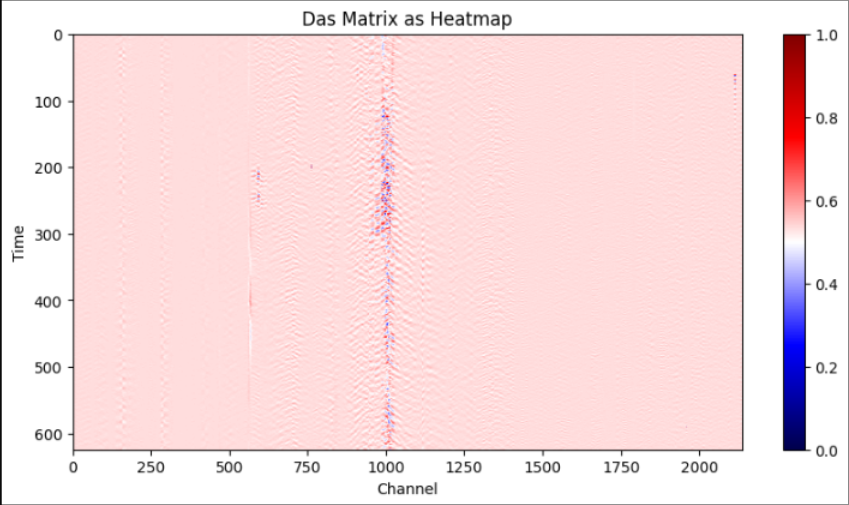
\includegraphics[width=0.7\linewidth]{figures/das_example.png}
    \caption{DAS data frame example}
    \label{fig:dasframe-ex}
\end{figure}

\acrshort{das} data can be stored in several different file formats. Data stored in \acrshort{hdf5} files have the advantage of storing additional metadata beside it and is ideal for complex datasets requiring extensive contextual information. Other formats such as TDMS are also structured around hierarchical data \cite{10.1145/800196.805973}, and is often used for storing \acrshort{das} data. Regardless of the chosen format, certain metadata are crucial for effectively handling and interpreting DAS data:

\textbf{Timestamps} is used for temporal alignment and analysis

\textbf{Gauge length} is the spatial resolution of measurements

\textbf{Channel decimation} stores information on spatial sampling. Not all channels along the total measurement is stored, and so to understand the location of a signal, the gauge length in combination with the channel decimation tells us the exact distance from the start of the measurement.

\textbf{Sample Rate} is the temporal resolution of the data, and is measured in hertz.

\acrshort{das} data itself is stored as a matrix, usually where the axis represent time and signal channels.

\begin{table}[!h]
\centering
\begin{equation*}
\mathbf{X} = \begin{bmatrix}
x_{1,1} & x_{1,2} & \cdots & x_{1,n-1} & x_{1,n} \\
x_{2,1} & x_{2,2} & \cdots & x_{2,n-1} & x_{2,n} \\
\vdots & \vdots & \ddots & \vdots & \vdots \\
x_{t-1,1} & x_{t-1,2} & \cdots & x_{t-1,n-1} & x_{t-1,n} \\
x_{t,1} & x_{t,2} & \cdots & x_{t,n-1} & x_{t,n}
\end{bmatrix}
\end{equation*}
\label{fig:dasmatrix}
\end{table}

In the matrix $\textbf{X}$ above, $t$ denotes the number of recordings for the file; for one second this would be equal to the sample rate. $n$ is the amount of channels stored. To process this data as fast as possible, it is important to consider which memory alignment the programming language of choice uses. In Julia, MatLab and Fortran, memory is stored in column-major order, while in most other languages, memory is stored in a row-major order. 

\subsection{Radio Frequency Filtering}

\acrfull{rf} filtering is of paramount importance in \acrshort{das} and \acrfull{dsp}. The signal quality can be improved by removing unnecessary noise from the data, and can decrease the overall of signal loss. In general, there are four types of filters, and can be defined as follows:

\begin{itemize}
    \item \textit{Band-pass filters} only allows frequencies between two cutoff frequencies $F_{low}$ and $F_{high}$
    \item \textit{Band-stop filters} stops frequencies between two cutoff frequencies $F_{low}$ and $F_{high}$
    \item \textit{Low-pass filters} only allows frequencies above the cut-off frequency $F_{low}$
    \item \textit{High-pass filters} only allows frequencies above the selected frequency $F_{high}$
\end{itemize}

A common approach to preprocessing \acrshort{das} data usually involves applying a bandpass to the signal matrix. Due to \acrshort{das} data being sensitive and capturing a broad range of frequencies, it is beneficial to limit the signals to a range of interest, depending on domain and application.

\vspace{0.5cm}

\begin{figure}[!h]
    \centering
    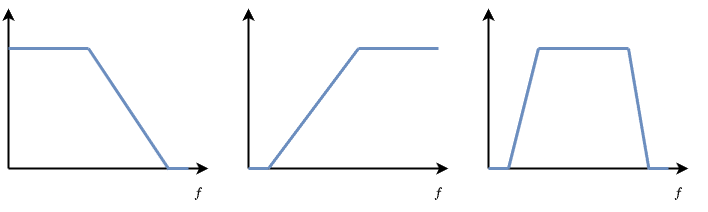
\includegraphics[width=0.8\linewidth]{figures/lowhighpass.png}
    \caption{Low-, High- and Band-pass filters}
    \label{fig:rffilters}
\end{figure}


\subsection{Tukey Window}
\label{dsp:tukey}

Window functions are function often used in \acrshort{dsp} to avoid artifacts. This is done by setting values outside a pre-defined interval to zero and apply a taper from the pass-band to the first zero-value. The Tukey window \cite{tukey1967introduction}, also known as the \textit{cosine-tapered window} is a common approach to reduce edge effects, and is defined as follows:

\[
    w(x)= 
\begin{cases}
    \frac{1 + \cos{2 \pi \alpha (x + \frac{1-\alpha}{2})}}{2}, & \text{if } x \leq \frac{1-\alpha}{2}\\
    1,              & \text{if } \frac{\alpha}{2} < x \leq \frac{\alpha}{2}\\
    \frac{1 + \cos{2 \pi \alpha (x - \frac{1-\alpha}{2})}}{2}, & \text{if } x > \frac{1-\alpha}{2}
\end{cases}
\]

This window becomes a rectangle when $\alpha = 0$.


\subsection{Resampling}

Resampling, also known as sampling-frequency conversion, is the act of modifying the sampling rate of a discrete signal to obtain a new discrete representation of this data. In many applications, particularly those involving \acrshort{dsp}, data is often initially collected at a very high sampling rate to capture fine details. However, for subsequent analysis, or storage, this high sampling rate may not be necessary or efficient. Down-sampling, also known as decimation, is a form of resampling where the sampling rate is reduced, can be applied to:

\begin{itemize}
    \item Decrease memory consumption for data storage
    \item Reduce computational time for data processing
    \item Balance the trade-off between processing efficiency and data resolution
\end{itemize}

By reducing the sampling rate, one may retain the essential characteristics of the data while reducing data volume and computational requirements. However, one must be careful to avoid aliasing, and ensure that the resampled data represents the phenomena of interest. 

\subsubsection{Parallel Channel Decimation}

\acrshort{das} data is a prime candidate for down-sampling due to its often high sampling rate. This operation is often referred to as \textit{channel decimation}. Channel decimation applies down-sampling on a per-channel level to decrease memory consumption. This operation can be deemed \textit{trivial parallizable} by the fact that each channel can be down-sampled independently. By introducing $P$ workers, each worker $P_i$ can down-sample a chunk of channels in parallel. Consequentially, the resulting outputs can be concatenated into a new matrix. This operation can be described as follows:

\[
A = \begin{bmatrix}
a_{11} & a_{12} & \cdots & a_{1n} \\
a_{21} & a_{22} & \cdots & a_{2n} \\
\vdots & \vdots & \ddots & \vdots \\
a_{m1} & a_{m2} & \cdots & a_{mn}
\end{bmatrix}
\]

%\vspace{1cm}

\begin{center}
Resample each column in parallel
\end{center}

%\vspace{0.5cm}

\[
B = \begin{bmatrix}
b_{11} & b_{12} & \cdots & b_{1n} \\
b_{21} & b_{22} & \cdots & b_{2n} \\
\vdots & \vdots & \ddots & \vdots \\
b_{h1} & b_{h2} & \cdots & b_{hn}
\end{bmatrix}
\]

In the equation above, $A$ is the input matrix of size $m \times n$.  $B$ is the resultant matrix, where $h$ is calculated as follows: 

$$h = m \times rate = m \times \dfrac{F_{target}}{F}$$

$m$ is the number of rows, which in the case of a \acrshort{das} signal where the channels are stored column-wise, can be defined by the sample frequency $F$ multiplied by the signal duration $dur$ in seconds.